
\begin{frame}
	\frametitle{Copter Rotation}
		\begin{figure}[p]
			\centering
			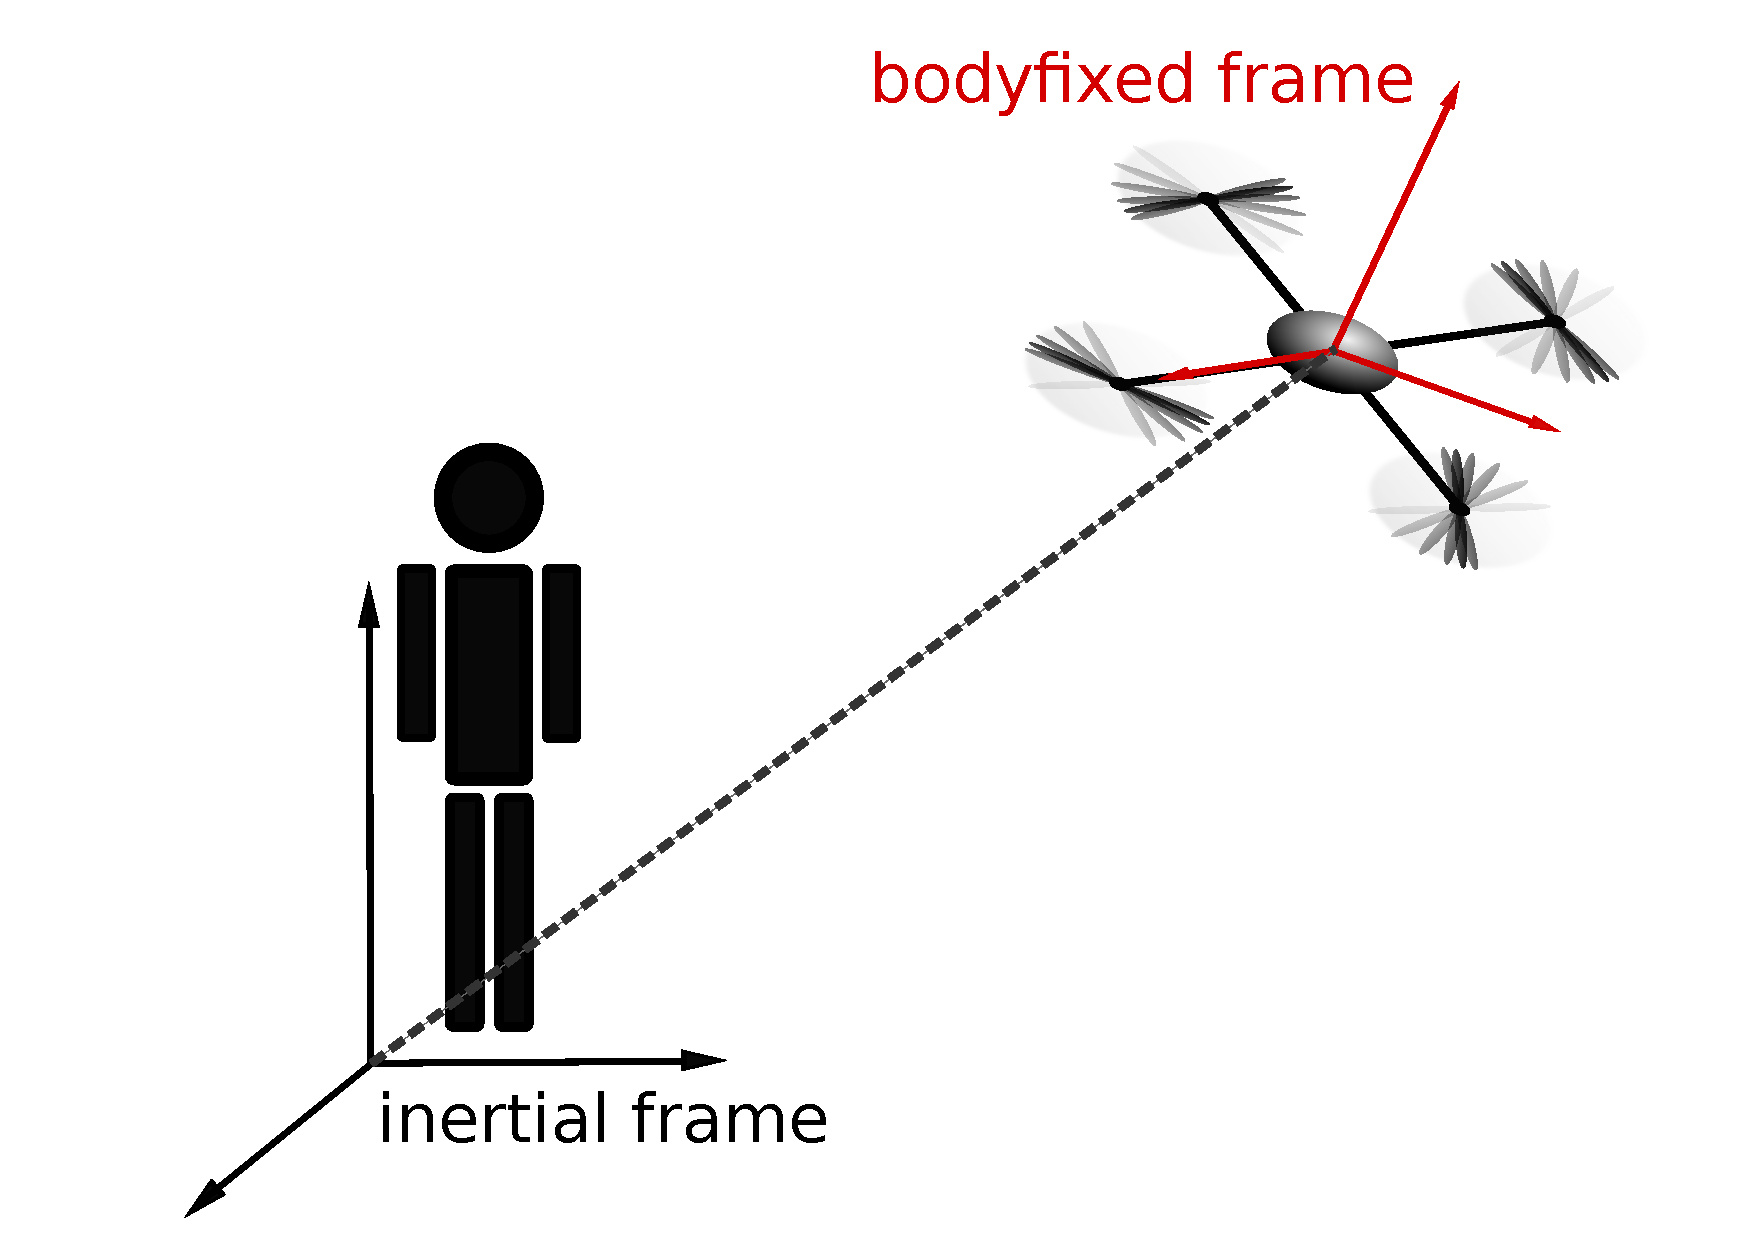
\includegraphics[width=0.8\textwidth]{images/Koordinatensysteme.pdf}
			\label{fig:Koordinatensysteme}
	\end{figure}
\end{frame}

%\begin{frame}
	%\frametitle{Quaternions}
	%\begin{block}{}
		%\centering
		%\vspace{1ex}
		%\( q = a + \textup{i}b+\textup{j}c+\textup{k}d \qquad a, b, c, d \in \mathbb{R} \)
		%\vspace{1ex}
	 %\end{block}
	%\end{frame}

\begin{frame}
	\frametitle{Quaternions}
	\begin{block}{}
		\centering
		\( q = a + \textup{i}b+\textup{j}c+\textup{k}d \qquad a, b, c, d \in \mathbb{R} \) \\
		\vspace{.5ex}
		\(\Leftrightarrow\) \\
		\vspace{1ex}
		\( \hspace{1ex} q = \begin{pmatrix} a \\ b \\ c\\ d \end{pmatrix} \in \mathbb{R}^4 \)
	\end{block}
	
	\vspace{1em}
			\onslide<2-> \centering
			represent rotation \( \quad \Leftrightarrow \quad \Vert q \Vert = 1 \quad \Leftrightarrow \quad q \in \mathcal{S}^3\) 
\end{frame}

\begin{frame}
	\frametitle{Drift Correction}
		\begin{columns}[T] % align columns
			\begin{column}{.55\textwidth}
			\centering
				\begin{textblock}{0}(-4.4,-5)
					\begin{tikzpicture}[scale=4]

	%Colors
	\definecolor{red}{RGB}{190,0,0};
  
  % Styles
  %\tikzstyle{axes}=[->]
	\tikzstyle{every node}=[font=\normalsize]

  % The graphic
  \draw[style=help lines,step=1cm] (-1.2,0) (1.2,1.2);
  \draw[thick] (0,0) (0:1cm) arc (0:98:1cm) ;
    
  \begin{scope}%[style=axes]
    \draw[thick,->] (-.2,0) -- (1.2,0) node[anchor=west] {};
    \draw[thick,->] (0,-.2) -- (0,1.5) node[anchor=west] {};

    \foreach \x/\xtext in {1}
      \draw[xshift=\x cm] (0pt,1pt) -- (0pt,-1pt) node[below,fill=white] {$\xtext$};
		\foreach \y/\ytext in {1}
      \draw[yshift=\y cm] (0pt,1pt) -- (0pt,-1pt) node[left=5pt,fill=white] {$\ytext$};
  \end{scope}
  
  \node at (25:1cm) (q0) [circle, draw, fill=black, inner sep = 0.07cm]{};
	\node[right=3pt] at (25:1cm) {$q_0$};
	\node at (0.5cm,1.294cm) (q1) [circle, draw, fill=black, inner sep = 0.07cm]{};
	\node<1>[right=3pt] at (q1) {$q_1=q_0+\Delta h\cdot \dot{q}_0$};
	\draw<1>[red, thick,->] (q0) to (q1);
	
	\node<2>[right=3pt] at (0.5cm,1.281cm) {$q_1$};
	\draw<2>[thick] (q0) to (q1);
	\node<2> at (68.87:1cm) (q1_normed) [circle, draw, fill=black, inner sep = 0.07cm]{};
	\node<2>[below=5pt] at (68.87:1cm) {$\mathlarger{\frac{q_1}{\|q_1\|}}$};
		\draw<2>[dashed,red,thick,->] (q1) -- (q1_normed) node[anchor=west] {};
\end{tikzpicture}
				\end{textblock}
			\end{column}
			\hfill
			\begin{column}{0.45\textwidth}
				\begin{textblock}{.963\columnwidth}(0,0)
					\begin{block}{}
					\centering
						\( \dot{q}(t) = \tilde{f}(q(t))\only<2->{-\lambda(q(t))} \)
					\end{block}
				\end{textblock}
				\end{column}
		\end{columns}
\end{frame}

%\begin{frame}
	%\frametitle{Drift Correction}
		%\begin{columns}[T] % align columns
			%\begin{column}{.55\textwidth}
				%\begin{textblock}{0}(-4.4,-5)
					%\begin{tikzpicture}[scale=4]

	%Colors
	\definecolor{red}{RGB}{190,0,0};
  
  % Styles
  %\tikzstyle{axes}=[->]
	\tikzstyle{every node}=[font=\normalsize]

  % The graphic
  \draw[style=help lines,step=1cm] (-1.2,0) (1.2,1.2);
  \draw[thick] (0,0) (0:1cm) arc (0:98:1cm) ;
    
  \begin{scope}%[style=axes]
    \draw[thick,->] (-.2,0) -- (1.2,0) node[anchor=west] {};
    \draw[thick,->] (0,-.2) -- (0,1.5) node[anchor=west] {};

    \foreach \x/\xtext in {1}
      \draw[xshift=\x cm] (0pt,1pt) -- (0pt,-1pt) node[below,fill=white] {$\xtext$};
		\foreach \y/\ytext in {1}
      \draw[yshift=\y cm] (0pt,1pt) -- (0pt,-1pt) node[left=5pt,fill=white] {$\ytext$};
  \end{scope}
  
  \node at (25:1cm) (q0) [circle, draw, fill=black, inner sep = 0.07cm]{};
	\node[right=3pt] at (25:1cm) {$q_0$};
	\node at (0.5cm,1.294cm) (q1) [circle, draw, fill=black, inner sep = 0.07cm]{};
	\node[right=3pt] at (0.5cm,1.294cm) {$q_1$};
	\draw[thick] (q0) to (q1);
	\node at (68.87:1cm) (q1_normed) [circle, draw, fill=black, inner sep = 0.07cm]{};
	\node[below=5pt] at (68.87:1cm) {$\mathlarger{\frac{q_1}{\|q_1\|}}$};
	\draw[dashed,red,thick,->] (q1) -- (q1_normed) node[anchor=west] {};
\end{tikzpicture}
				%\end{textblock}
			%\end{column}
			%\hfill
			%\begin{column}{0.45\textwidth}
				%\begin{textblock}{.9\columnwidth}(0,0)
					%\begin{block}{}
					%\centering
					%\( \dot{q}(t) = \tilde{f}(q(t))\only<2->{-\lambda(q(t))} \)
					%\end{block}
				%\end{textblock}
				%\end{column}
		%\end{columns}
%\end{frame}